\section{Opportunistic Monitoring}
\label{sec:monitoring_hard_drop.drop}

In this section we present a framework for opportunistically performing
monitoring in such a way as to ensure that the main task's execution time does
not exceed its WCET bound. The basic idea is that on a monitoring event, the
system checks whether there is enough slack to account for the worst-case
impact of monitoring on the main task's execution time. If there is enough
slack, then the monitoring task proceeds. If there is not enough slack, then
instead the event is dropped. 

There are two main challenges in this scheme. The first is how to measure slack
at run time and decide when it is necessary to drop monitoring tasks, which we
discuss in Section~\ref{sec:monitoring_hard_drop.drop.slack}. Once it has been
decided to drop a monitoring event, the second issue is how to drop the
monitoring task in such a way as to maintain the correctness of the monitoring
scheme which we discuss in
Section~\ref{sec:monitoring_hard_drop.drop.dropping_tasks}.

\subsection{Measuring Slack}
\label{sec:monitoring_hard_drop.drop.slack}

% Shows execution time and slack
\begin{figure}
  \begin{center}
    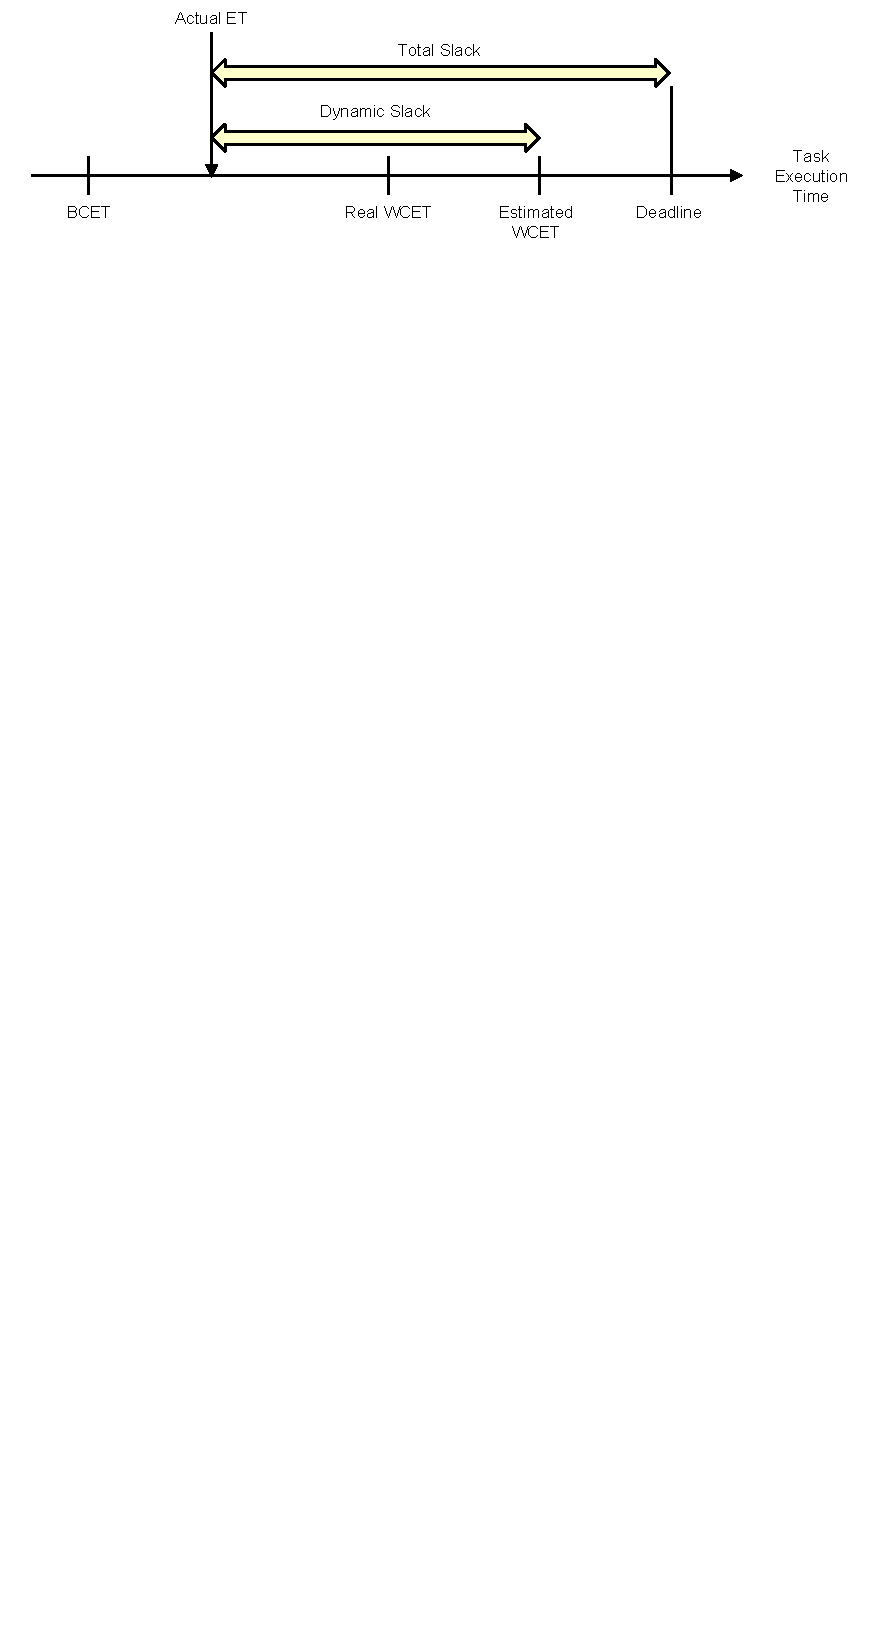
\includegraphics{monitoring_hard_drop/figs/slack_defn.pdf}
    \caption{Dynamic slack and total slack.}
    \label{fig:monitoring_hard_drop.drop.slack_defn} 
  \end{center}
\end{figure}

In order to decide when it is possible to perform monitoring, we must be able
to measure the dynamic slack available.  Dynamic slack is defined as the
difference between a task's expected worst-case execution time (WCET) and its
actual execution time \cite{anantaraman-multi_task_visa-rtss04}. This is only a
portion of the total slack which is the difference between a task's finish time
and its deadline (see Figure~\ref{fig:monitoring_hard_drop.drop.slack_defn}).
Although the dynamic slack only accounts for a portion of the total slack, we
only focus on dynamic slack because this is the portion of slack that is
specific to a task.  Additional slack in the schedule could be assigned to a
specific task to be used for monitoring by the system designer or scheduler.
For brevity, we will use the term slack to refer to dynamic slack.

% Diagram showing sub-tasks and slack accumulation/usage
\begin{figure}
  \begin{center}
    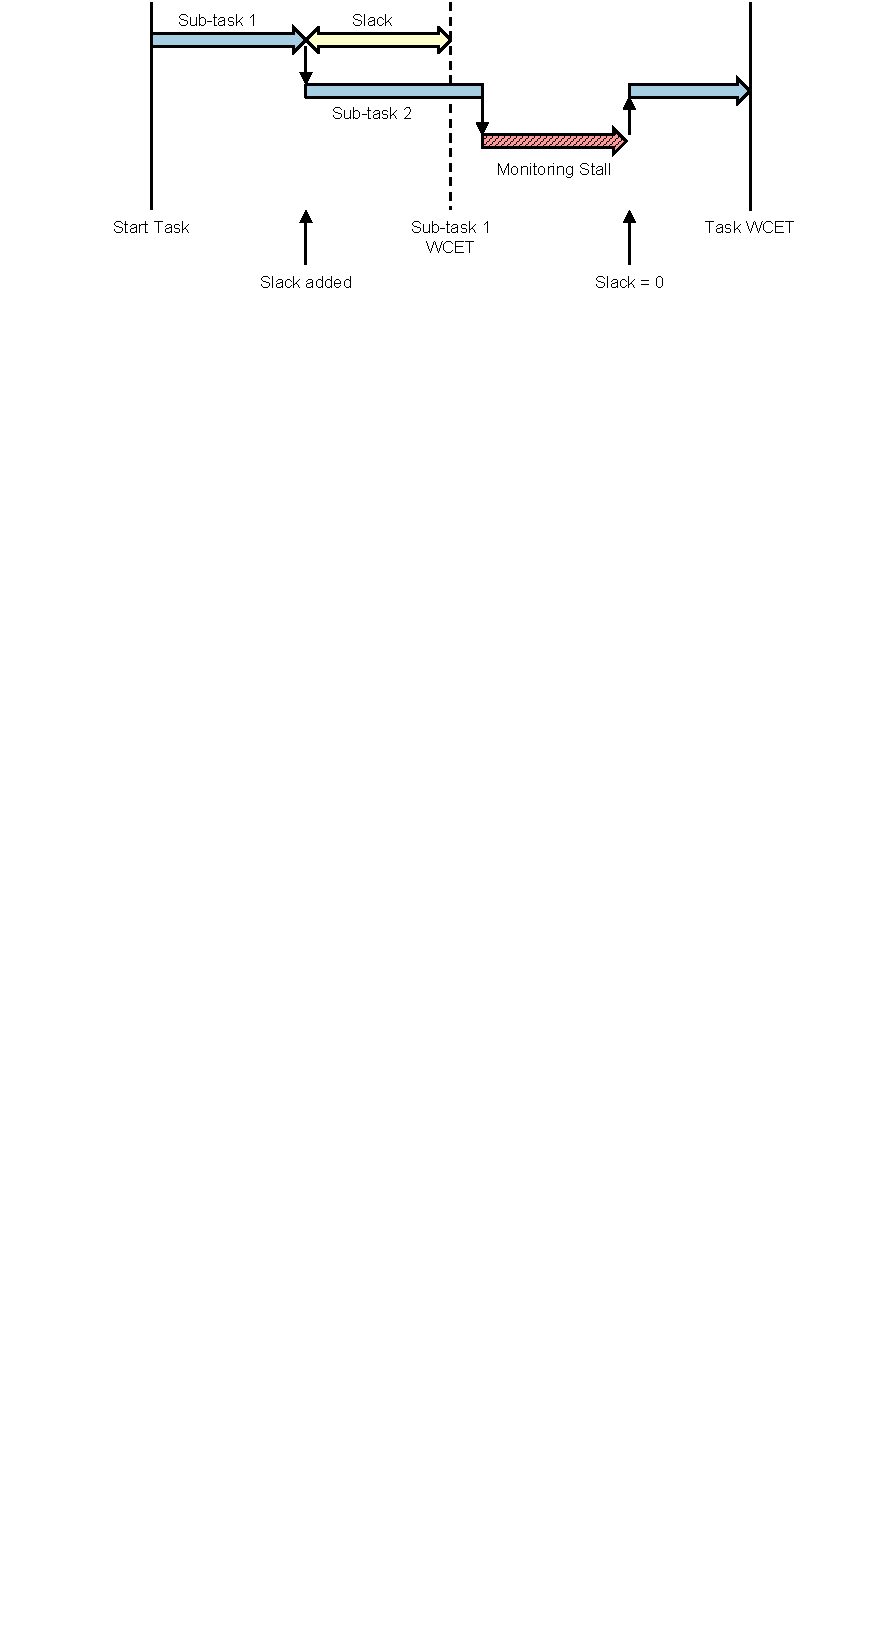
\includegraphics{monitoring_hard_drop/figs/task_slack.pdf}
    \caption{Dynamic slack increases when a sub-task finishes early. Slack is
    consumed as monitoring causes the task to stall.}
    \label{fig:monitoring_hard_drop.drop.task_slack} 
  \end{center}
\end{figure}

In order to perform monitoring as the task runs, we need to be able to measure
dynamic slack as the task runs.  We can track dynamic slack by setting a number
of checkpoints throughout the task.  These checkpoints effectively divide the
task into a number of sub-tasks.  For each of these sub-tasks, the sub-task's
WCET is determined.  At run-time when a sub-task finishes, the difference
between its actual run-time and its WCET is the slack generated by the
sub-task.  Specifically, we insert code to mark each sub-task boundary.  At the
beginning of a sub-task, the WCET of a sub-task is loaded into a timer. Each
cycle, the timer decreases. At the end of a sub-task, the remaining value in
the timer is the slack generated by the sub-task. This value is added to the
current slack.  An example of this process is shown in
Figure~\ref{fig:monitoring_hard_drop.drop.task_slack}. In our experiments, the
division of a task into sub-tasks was done by hand but this process could be
automated to divide a task using function boundaries, code length, or some
other criteria.  In addition to the slack accumulated while running, a portion
of \emph{headstart slack} can be initially assigned by the designer or
scheduler to the task. For example, if the designer knows that static slack
exists in the schedule, this slack can be added to the initial dynamic slack of
a task to be used for monitoring.

By accumulating this slack as the task runs, we can determine whether
monitoring can be performed while still meeting the real-time constraints. If
the worst-case impact of a monitoring task on the main task is less than the
accrued slack, then the monitoring task can execute.  If running the monitoring
task causes the main task to stall, as in the example shown in
Figure~\ref{fig:monitoring_wcet.monitoring.pipeline}, then slack is consumed.
Slack was initially generated since the main task was running ahead of its
WCET, so stalling up to the slack time will not cause the main task to exceed
its WCET (see Figure~\ref{fig:monitoring_hard_drop.drop.task_slack}). In the
best case, the monitoring task executes entirely in parallel and does not
affect the main task and thus consumes no slack. On the other hand, if the
worst-case impact of the monitoring task on the main task's execution time is
greater than the slack, then, conservatively, the monitoring task cannot be
run. Instead, it must be dropped in order to guarantee that the main task
finishes within its WCET.

\subsection{Dropping Tasks}
\label{sec:monitoring_hard_drop.drop.dropping_tasks}

Dropping a monitoring task implies that some functionality of the monitor has
been lost.  This may cause either false negatives, where an error that occurs
in the main task's execution is not detected, or false positives, where the
monitor incorrectly believes an error has occurred.  For example, a false
positive can occur for UMC if a store monitoring event is dropped. This causes
the memory location of the store to not be marked as initialized. A subsequent
load for the memory location will incorrectly cause an error to be raised.  We
accept false negatives as the loss in coverage that we trade off in order to
ensure the WCET of the main task is met. However, we must safely drop
monitoring events in such a way as to avoid false positives so that the system
does not incorrectly raise an error.

% Need for a dropping task to prevent false positives.
In order to ensure that no false positives occur, we need to run a
\emph{dropping task} when a monitoring task is dropped.  The specifics of how
this dropping task operates may vary for different monitoring schemes. However,
in analyzing various monitoring schemes, we found that most monitoring tasks
perform operations of primarily two types: \emph{checks} and \emph{metadata
updates}. Monitoring tasks \emph{check} certain properties to ensure correct
main task execution and they \emph{update} metadata for bookkeeping. Skipping a
check operation can only cause false negatives and will never cause a false
positive. Therefore, the dropping task may simply skip a check operation.
Skipping an update operation can cause false negatives but may also cause false
positives.  Essentially, when an update operation is skipped, we can no longer
trust the corresponding metadata. In some cases, the dropping task can handle
this by setting the metadata to a neutral value that will not cause false
positives (e.g., cleared or null). A more general solution is for the dropping
task to mark the corresponding metadata as invalid, to prevent future false
positives.

% WCET for SW vs. HW vs. neither scheme
\begin{figure}
  \begin{center}
    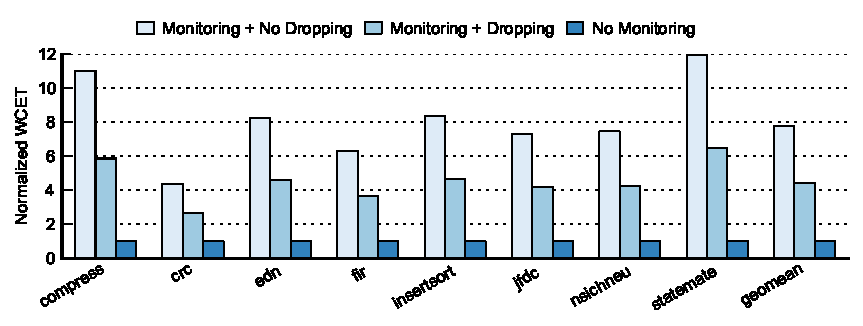
\includegraphics{monitoring_hard_drop/data/sw_drop_wcet.pdf}
    \caption{WCET with original monitoring task, with software dropping task,
    and with no monitoring for UMC. Results are normalized to the WCET with no
    monitoring.}
    \label{fig:monitoring_hard_drop.drop.sw_dropwcet} 
  \end{center}
\end{figure}

% Want to minimize WCET of dropping task
In the worst case, no monitoring can be done and the system must ensure that
there is enough time to run a dropping task for every monitoring event in order
to avoid false positives.  Thus, the main task's WCET estimation must be
modified to take into account the worst-case impact due to the dropping task.
By minimizing the dropping task's execution time, the impact on the main task's
WCET can be much lower than the impact due to the monitoring task.
Figure~\ref{fig:monitoring_hard_drop.drop.sw_drop_wcet} compares the original WCETs
with and without monitoring to the WCET with dropping tasks implemented in
software for UMC. The WCETs are normalized to the WCET without monitoring.  The
WCET with dropping is reduced by 43\% on average from the WCET without
dropping. 

